A tensão admissível de fadiga é dada pela equação:

\begin{equation}
  \sigma_{a_f} = \frac{\sigma_{f_a}}{K_f}
  \label{eq:sigma_a_f}
\end{equation}

Onde:

\begin{itemize}
  \item $\sigma_{a_f}$: tensão admissível de fadiga em \si{\mega\pascal}.
  \item $\sigma_{f_a}$: tensão limite de fadiga em \si{\mega\pascal}.
  \item $K_f$: fator de segurança à fadiga segundo a norma NBR 8400 \cite{nbr8400}.
\end{itemize}

\vspace{1em}

A tensão limite de fadiga é dada pela equação:

\begin{equation}
  \sigma_{f_a} = \num{0.5} \cdot \sigma_R
  \label{eq:sigma_f_a}
\end{equation}

Onde:

\begin{itemize}
  \item $\sigma_R$: tensão de resistência em \si{\mega\pascal} (Tabela \ref{tab:tensoes_eixo_do_tambor}).
\end{itemize}

\vspace{1em}

Substituindo os valores na equação \eqref{eq:sigma_f_a}:

\begin{align*}
  \sigma_{f_a} & = \num{0.5} \cdot 600            \\
  \sigma_{f_a} & = \boxed{\SI{300}{\mega\pascal}}
\end{align*}

Segundo a norma NBR 8400 \cite{nbr8400}, o fator de segurança à fadiga é dado por:

\begin{equation}
  K_f = K_s \cdot K_d \cdot K_u \cdot K_c
  \label{eq:k_f}
\end{equation}

Onde:

\begin{itemize}
  \item $K_s$: fator forma da peça nas vizinhanças do ponto considerado.
  \item $K_d$: fator de dimensão da peça.
  \item $K_u$: fator de rugosidade da superfície.
  \item $K_c$: fator de corrosão.
\end{itemize}

Para obter o valor de $K_s$, é necessário correlacionar a tensão de resistência com as dimensões do eixo, conforme o gráfico abaixo:

\begin{figure}[H]
  \centering
  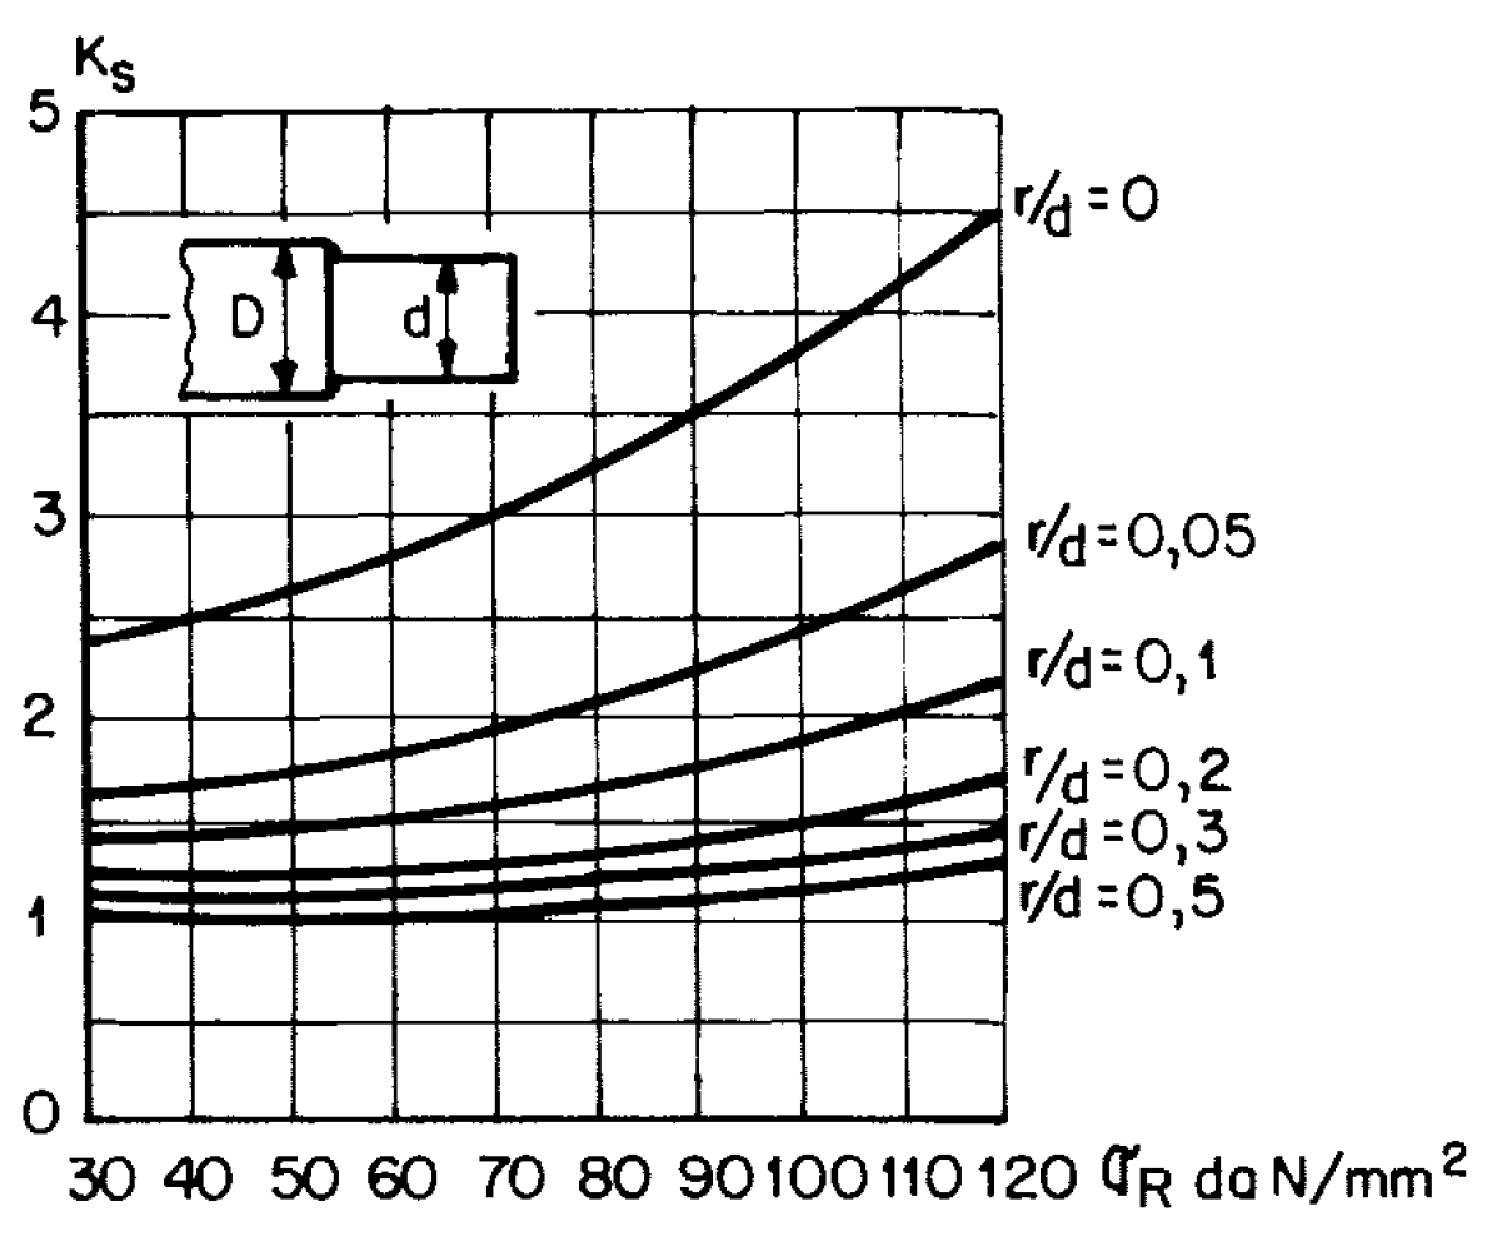
\includegraphics[width=0.5\textwidth]{content/sections/03_sistema_de_elevacao/sections/05_projeto_do_eixo_do_tambor/sections/02_verificacao_quanto_a_fadiga/figures/ks.pdf}
  \caption{Gráfico do fator $K_s$ segundo a norma NBR 8400 \cite[p.~106]{nbr8400}}
  \label{fig:k_s}
\end{figure}

A norma diz que o valor utilizado para selecionar a curva do gráfico é dado por $r/d + q$, onde $q$ pode ser obtido na tabela abaixo:

\begin{figure}[H]
  \centering
  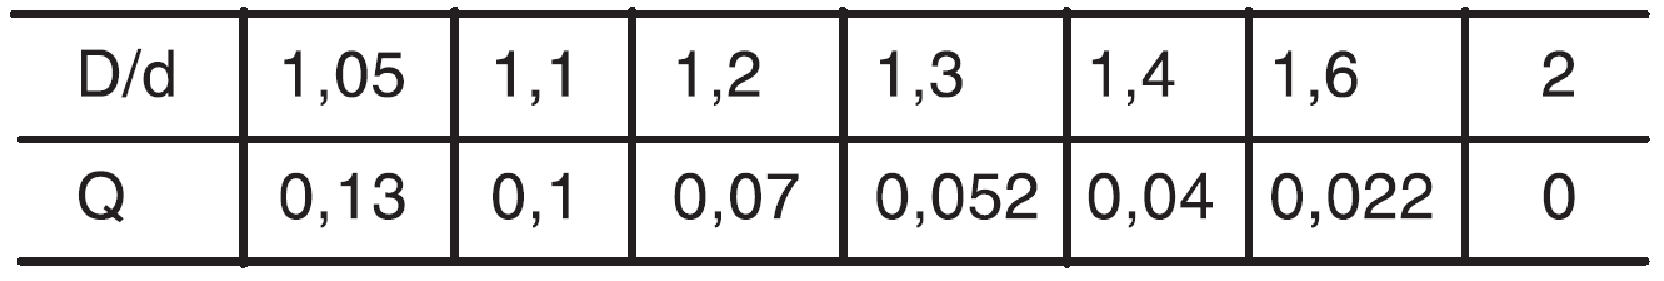
\includegraphics[width=0.5\textwidth]{content/sections/03_sistema_de_elevacao/sections/05_projeto_do_eixo_do_tambor/sections/02_verificacao_quanto_a_fadiga/figures/q.pdf}
  \caption{Tabela de valores de $q$ segundo a norma NBR 8400 \cite[p.~105]{nbr8400}}
  \label{fig:q}
\end{figure}

Calculando a razão entre os diâmetros do eixo:

\begin{align*}
  \frac{D}{d} & = \frac{d_e}{d}      \\
  \frac{D}{d} & = \frac{80}{70}      \\
  \frac{D}{d} & = \boxed{\num{1.14}}
\end{align*}

Para esse valor obtido, considera-se $q = \boxed{\num{0.07}}$.

Calculando a razão entre o raio e o diâmetro do eixo:

\begin{align*}
  \frac{r}{d} + q & = \frac{\num{1.5}}{\num{70}} + \num{0.07} \\
  \frac{r}{d} + q & \approx \boxed{\num{0.1}}
\end{align*}

Assim, é possível traçar os valores no gráfico e obter $K_s = \boxed{\num{1.5}}$.

\begin{figure}[H]
  \centering
  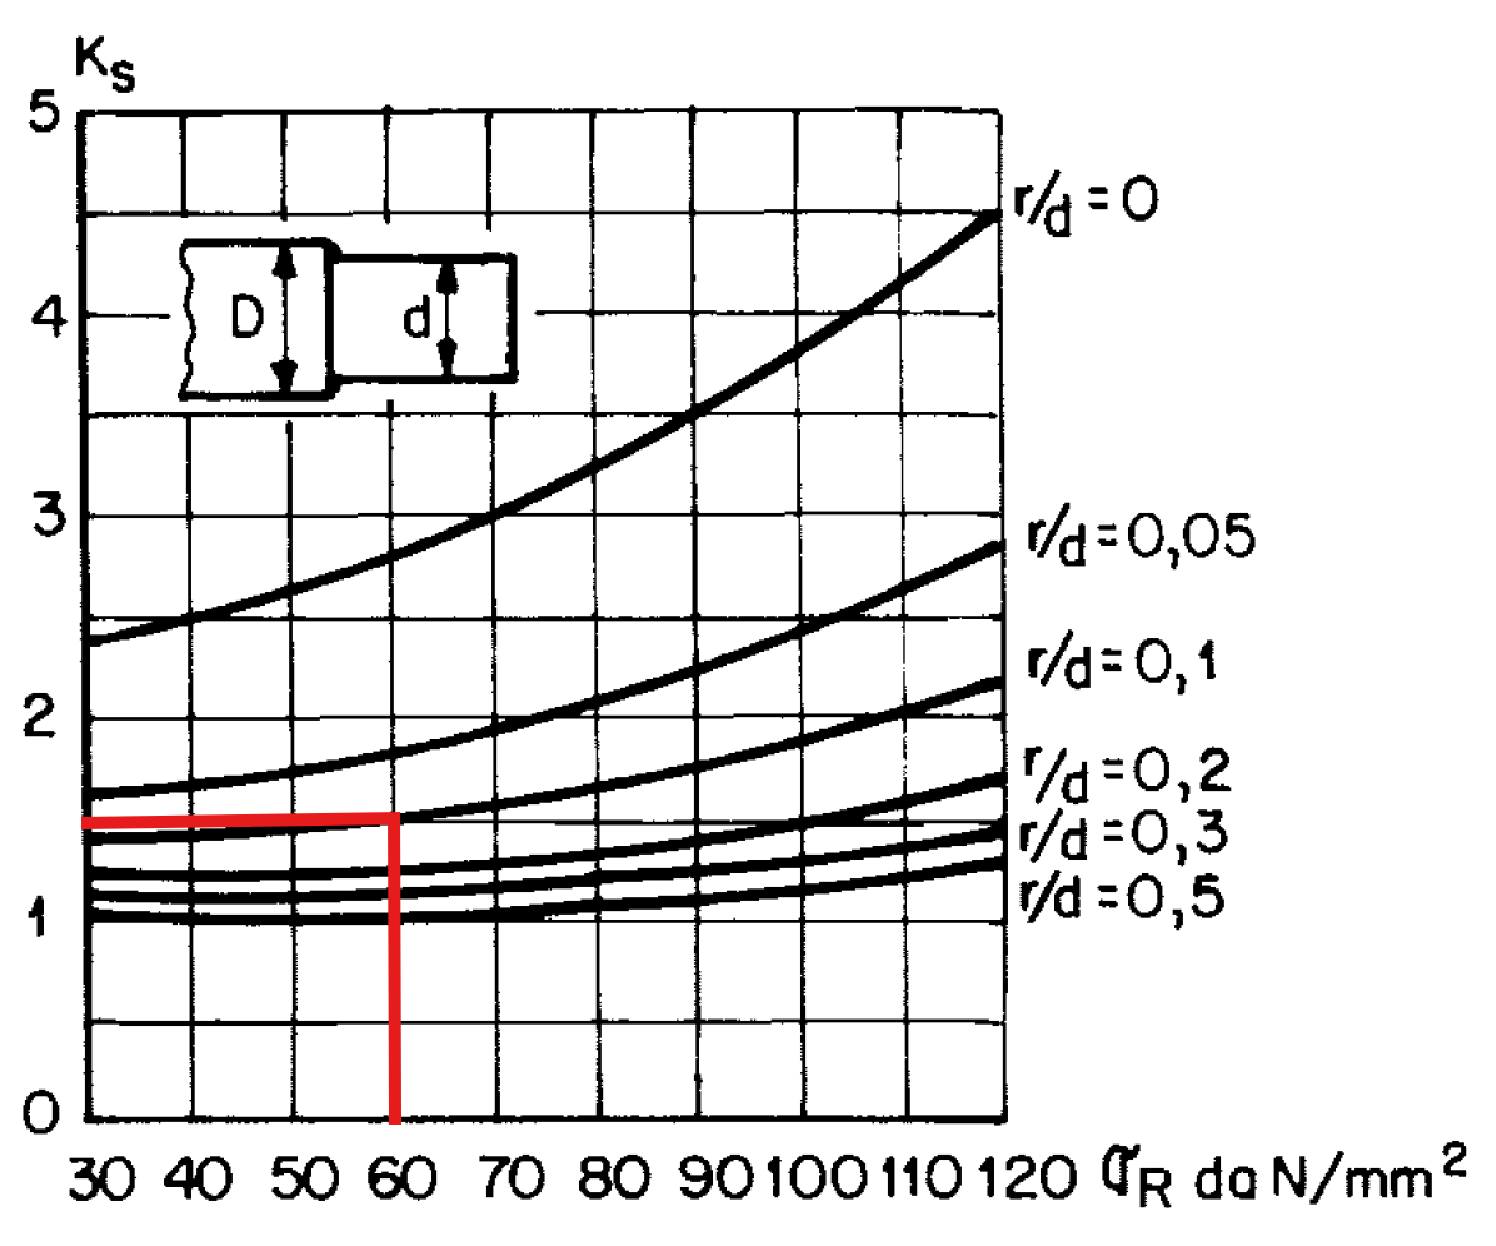
\includegraphics[width=0.5\textwidth]{content/sections/03_sistema_de_elevacao/sections/05_projeto_do_eixo_do_tambor/sections/02_verificacao_quanto_a_fadiga/figures/ks_tracado.pdf}
  \caption{Fator $K_s$ adotado \cite[p.~106]{nbr8400}}
  \label{fig:k_s_tracado}
\end{figure}

Segundo a norma, o fator de dimensão é obtido com base no diâmetro do eixo, conforme a tabela abaixo:

\begin{figure}[H]
  \centering
  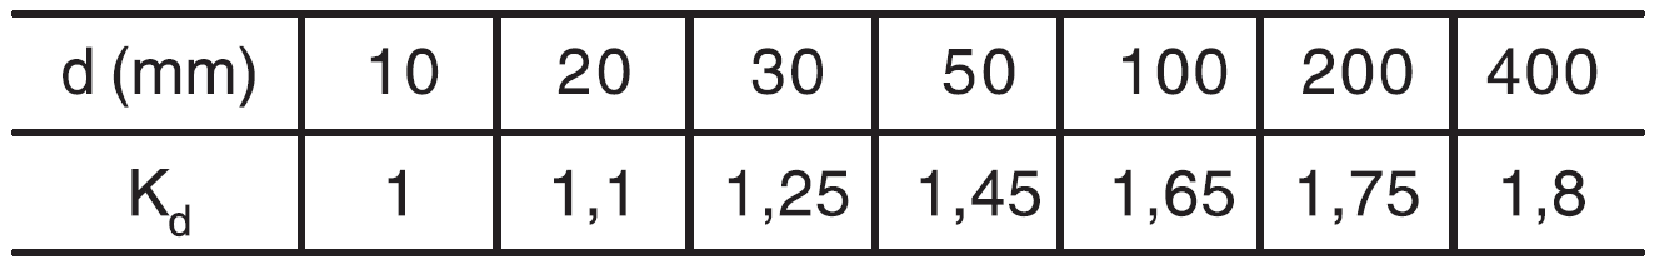
\includegraphics[width=0.5\textwidth]{content/sections/03_sistema_de_elevacao/sections/05_projeto_do_eixo_do_tambor/sections/02_verificacao_quanto_a_fadiga/figures/kd.pdf}
  \caption{Tabela de valores de $K_d$ segundo a norma NBR 8400 \cite[p.~105]{nbr8400}}
  \label{fig:k_d}
\end{figure}

Para o diâmetro do eixo adotado, $d = \boxed{\SI{100}{\milli\meter}}$, o fator de dimensão é $K_d = \boxed{\num{1.65}}$.

O fator de rugosidade da superfície, considerando uma superfície desbastada em torno, é $K_u = \boxed{\num{1.2}}$, conforme o gráfico abaixo:

\begin{figure}[H]
  \centering
  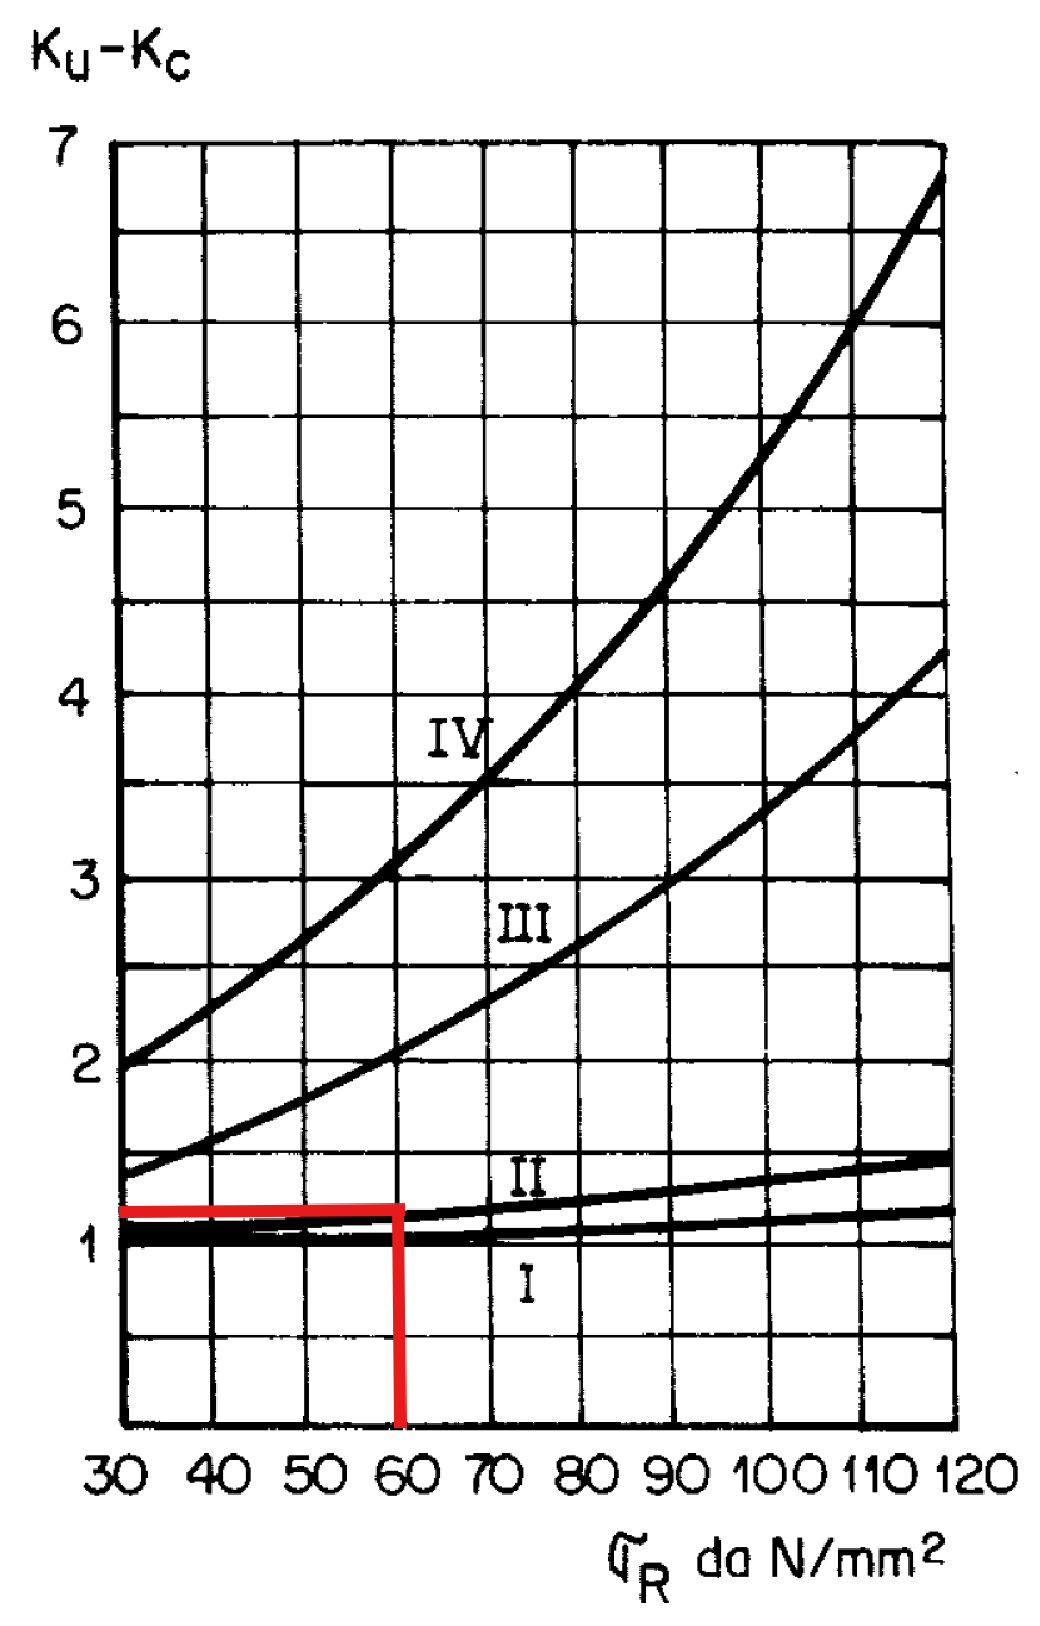
\includegraphics[width=0.5\textwidth]{content/sections/03_sistema_de_elevacao/sections/05_projeto_do_eixo_do_tambor/sections/02_verificacao_quanto_a_fadiga/figures/ku.pdf}
  \caption{Gráfico do fator $K_u$ segundo a norma NBR 8400 \cite[p.~107]{nbr8400}}
  \label{fig:k_u}
\end{figure}

O fator de corrosão, considerando que o eixo não será submetido a corrosão, pois estará fechado em ambiente coberto, é $K_c = \boxed{\num{1.0}}$.

Substituindo os valores na equação \eqref{eq:k_f}:

\begin{align*}
  K_f & = K_s \cdot K_d \cdot K_u \cdot K_c                          \\
  K_f & = \num{1.5} \cdot \num{1.65} \cdot \num{1.2} \cdot \num{1.0} \\
  K_f & = \boxed{\num{2.97}}
\end{align*}

Substituindo os valores na equação \eqref{eq:sigma_a_f}:

\begin{align*}
  \sigma_{a_f} & = \frac{\sigma_{f_a}}{K_f}          \\
  \sigma_{a_f} & = \frac{300}{\num{2.97}}            \\
  \sigma_{a_f} & = \boxed{\SI{101.01}{\mega\pascal}}
\end{align*}

A verificação quanto à fadiga é dada por:

\begin{equation}
  \delta \sigma_{c} \leq \sigma_{a_f}
  \label{eq:verificacao_fadiga}
\end{equation}

Onde:

\begin{itemize}
  \item $\delta$: coeficiente segundo a norma NBR 8400 \cite{nbr8400}.
  \item $\sigma_{c}$: tensão combinada em \si{\mega\pascal} \eqref{eq:tensao_combinada_tambor}.
  \item $\sigma_{a_f}$: tensão admissível de fadiga em \si{\mega\pascal} \eqref{eq:sigma_a_f}.
\end{itemize}

\vspace{1em}

O coeficiente $\delta$, considerando o grupo do mecanismo $1AM$, é $\delta = \boxed{\num{1.0}}$, conforme a tabela abaixo:

\begin{figure}[H]
  \centering
  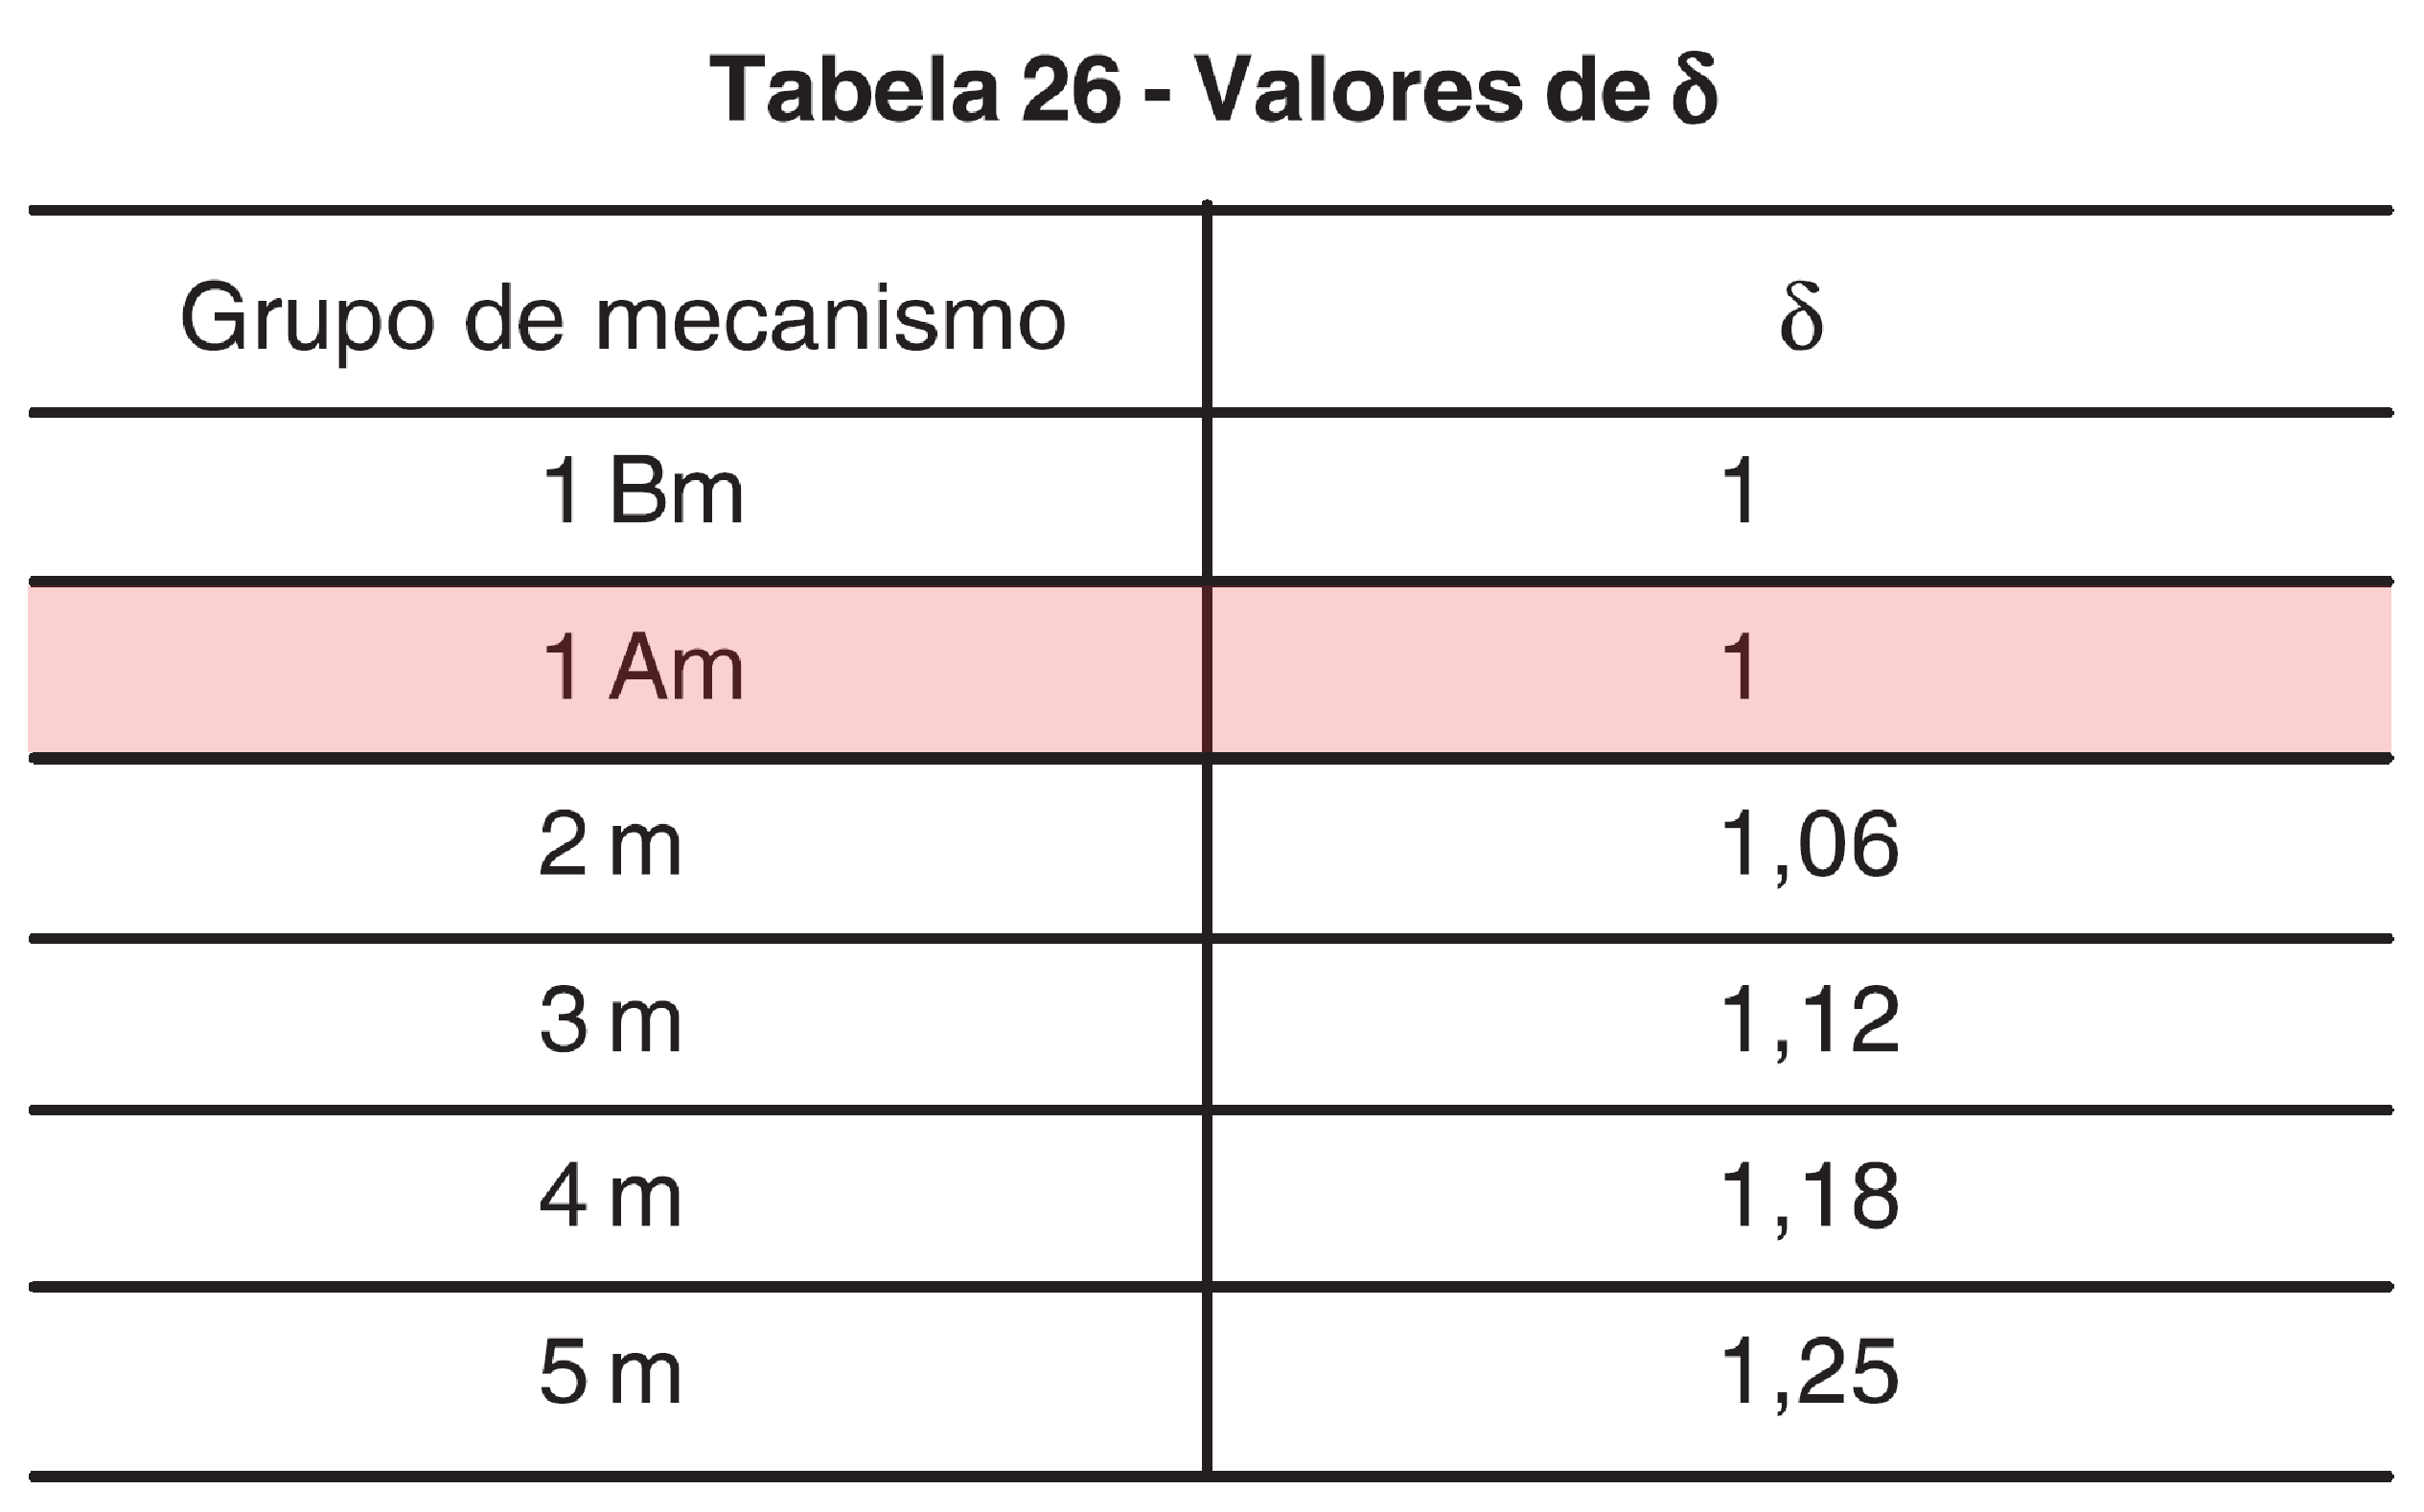
\includegraphics[width=0.5\textwidth]{content/sections/03_sistema_de_elevacao/sections/05_projeto_do_eixo_do_tambor/sections/02_verificacao_quanto_a_fadiga/figures/delta.pdf}
  \caption{Tabela de valores de $\delta$ segundo a norma NBR 8400 \cite[p.~32]{nbr8400}}
  \label{fig:delta}
\end{figure}

Verificando a condição de fadiga:

\begin{align*}
  \delta \sigma_{c}           & \leq \sigma_{a_f}                                    \\
  \num{1.0} \cdot \num{93.27} & \leq \num{101.01}                                    \\
  \SI{93.27}{\mega\pascal}    & \leq \SI{101.01}{\mega\pascal} \rightarrow \text{OK}
\end{align*}
